\begin{frame}
  \frametitle{Clustering images}

  \begin{center}
    Clustering is an \textit{unsupervised} learning task by which we
    look for structure in the data, grouping similar examples together
    \vskip20pt
    \only<1>{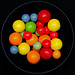
\includegraphics[height=0.25\textheight]{../../code/image_data/candy.jpg}}
    \only<2>{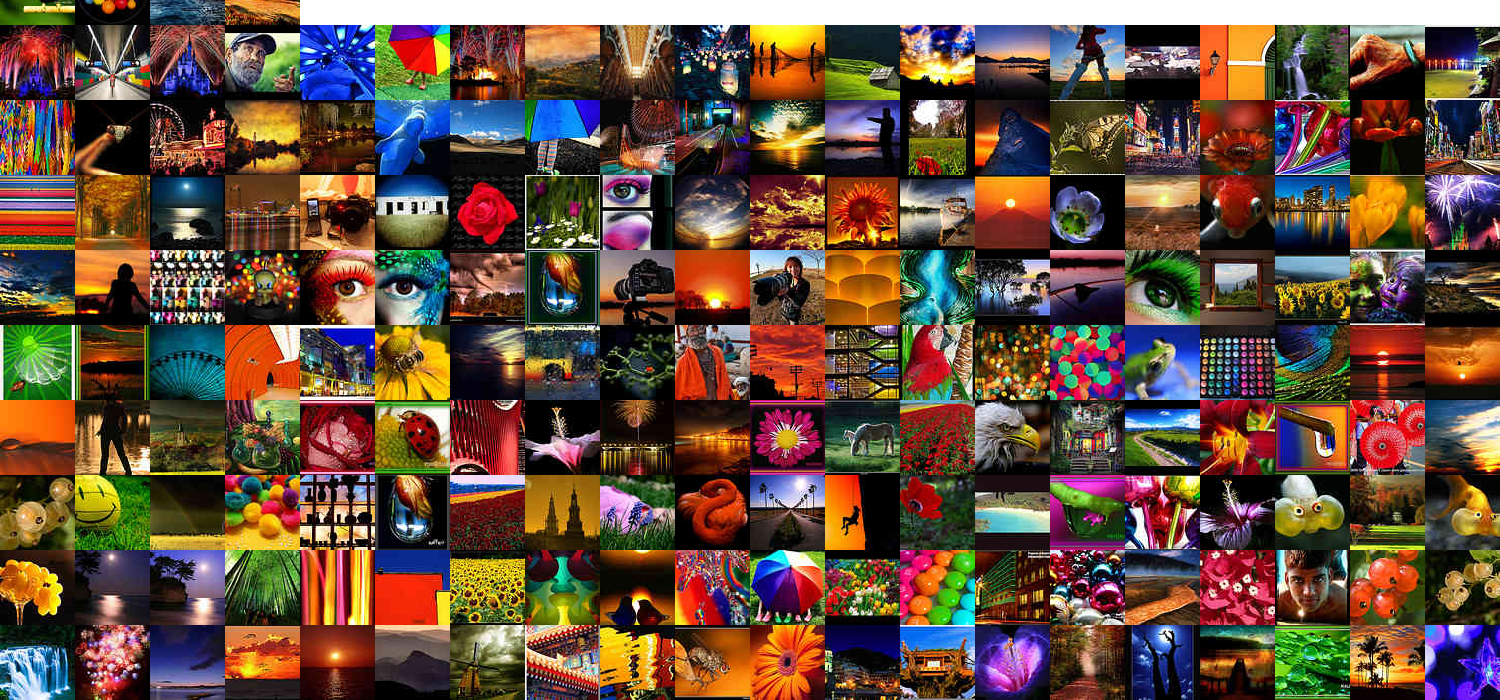
\includegraphics[height=0.25\textheight]{../../code/image_data/flickr_vivid_cluster_0}}
    \vskip20pt
    \only<1>{e.g., find groups of similar pixels within a single image}
    \only<2>{e.g., find groups of similar images across a collection of images}
  \end{center}

\end{frame}


\begin{frame}
  \frametitle{K-means clustering}

  \begin{center}
    K-means: represent each cluster by the average of its points 
    \vskip20pt
    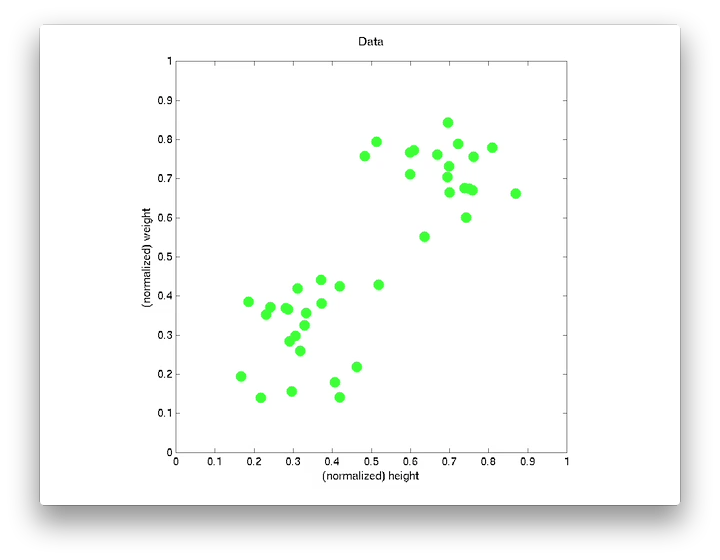
\includegraphics[width=0.6\textwidth]{em_animation_1.png}
    \vskip20pt
    Learn by iteratively updating cluster means and point assigments
  \end{center}
  % jntj: min inter-cluster var
\end{frame}

\begin{frame}[fragile]
  \frametitle{K-means clustering}

  \begin{center}

    \begin{columns}[c]
      
      \column{0.5\textwidth}
        K-means: \\
        \alert<1>{Choose number of clusters} \\
        \alert<1>{Initialize cluster centers} \\
        While not converged: \\
          \alert<2,4>{\hskip10pt Assign each point to closest cluster} \\
          \alert<3,5>{\hskip10pt Update cluster centers}

      \column{0.6\textwidth}

    \only<1>{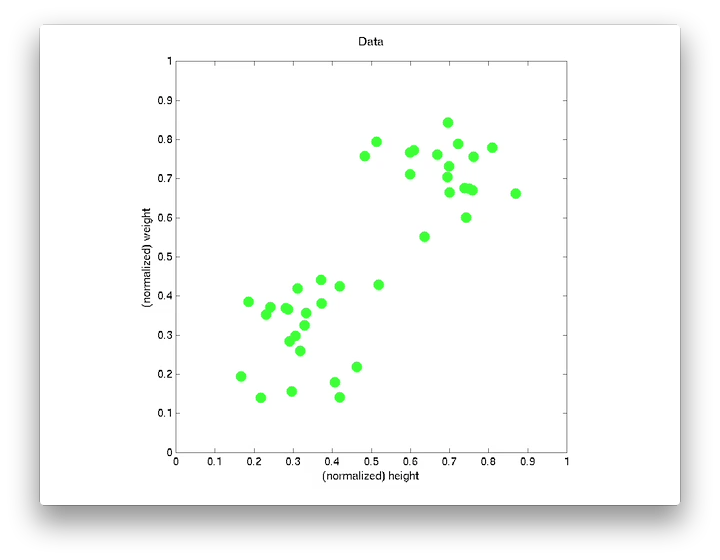
\includegraphics[width=1\textwidth]{em_animation_1.png}}
    \only<2>{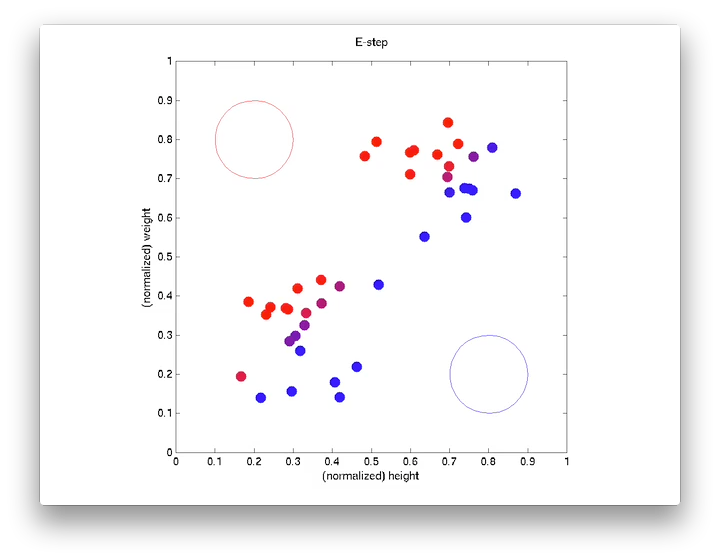
\includegraphics[width=1\textwidth]{em_animation_2.png}}
    \only<3>{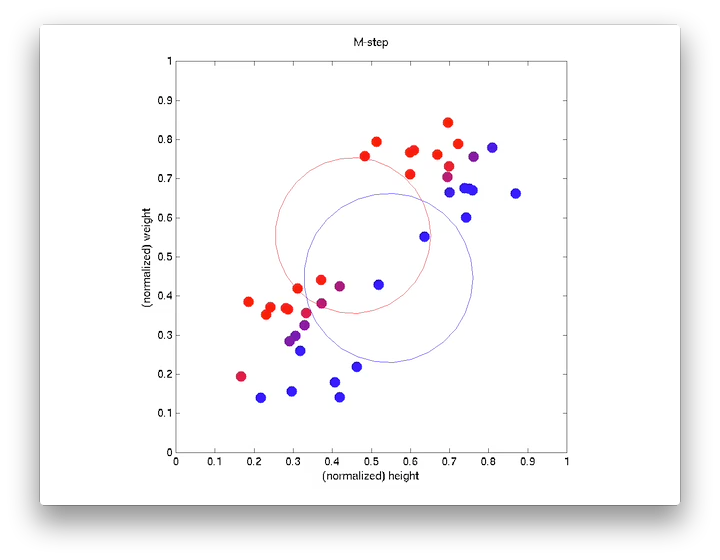
\includegraphics[width=1\textwidth]{em_animation_3.png}}
    \only<4>{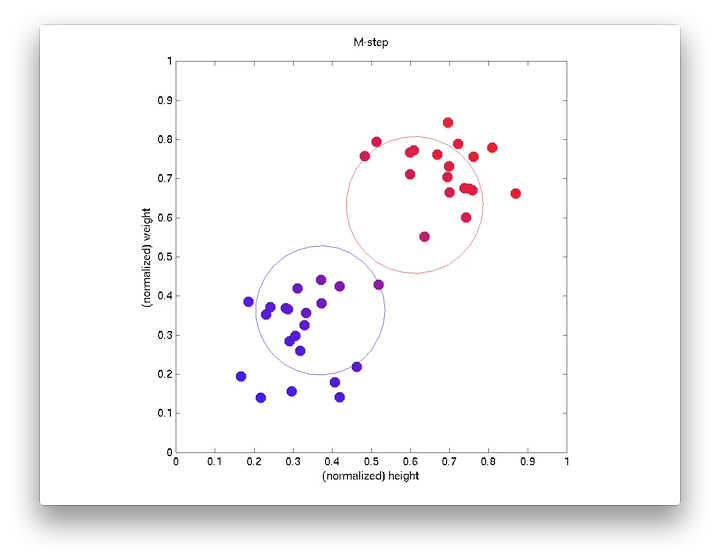
\includegraphics[width=1\textwidth]{em_animation_4.png}}
    \only<5>{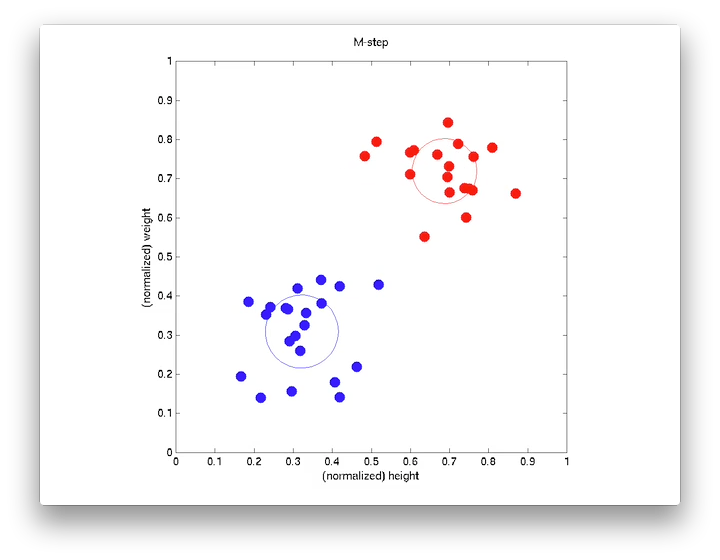
\includegraphics[width=1\textwidth]{em_animation_5.png}}

    \end{columns}
  \end{center}


\end{frame}


\begin{frame}
  \frametitle{Clustering pixels}

  \begin{center}
    Find groups of similar pixels within a single image \\
    (e.g. ``the bright red circles'')
    \vskip20pt
    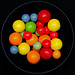
\includegraphics[height=0.25\textheight]{../../code/image_data/candy.jpg}
    \vskip20pt
    Represent each pixel as a separate example \\
    with its (R,G,B) value as a 3-d feature vector
  \end{center}

\end{frame}


\begin{frame}[fragile]
  \frametitle{Clustering pixels}

  \begin{center}

    \begin{block}{Group pixels within candy.jpg into 7 clusters}
        \begin{lstlisting}[language=bash]
 ./cluster_pixels.py candy.jpg 7
        \end{lstlisting}
    \end{block}
    \vskip20pt
    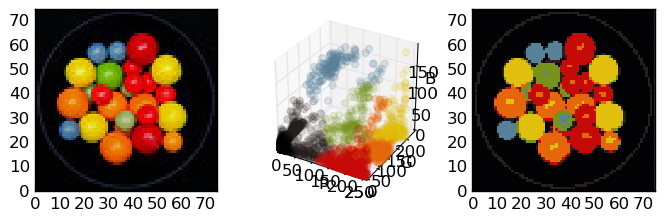
\includegraphics[width=\textwidth]{../../code/image_data/candy_clustered.png}
  \end{center}

\end{frame}

\begin{frame}
  \frametitle{Clustering images}

  \begin{center}
    Find groups of similar images within a collection of images \\
    (e.g. ``warm sunsets'')
    \vskip20pt
    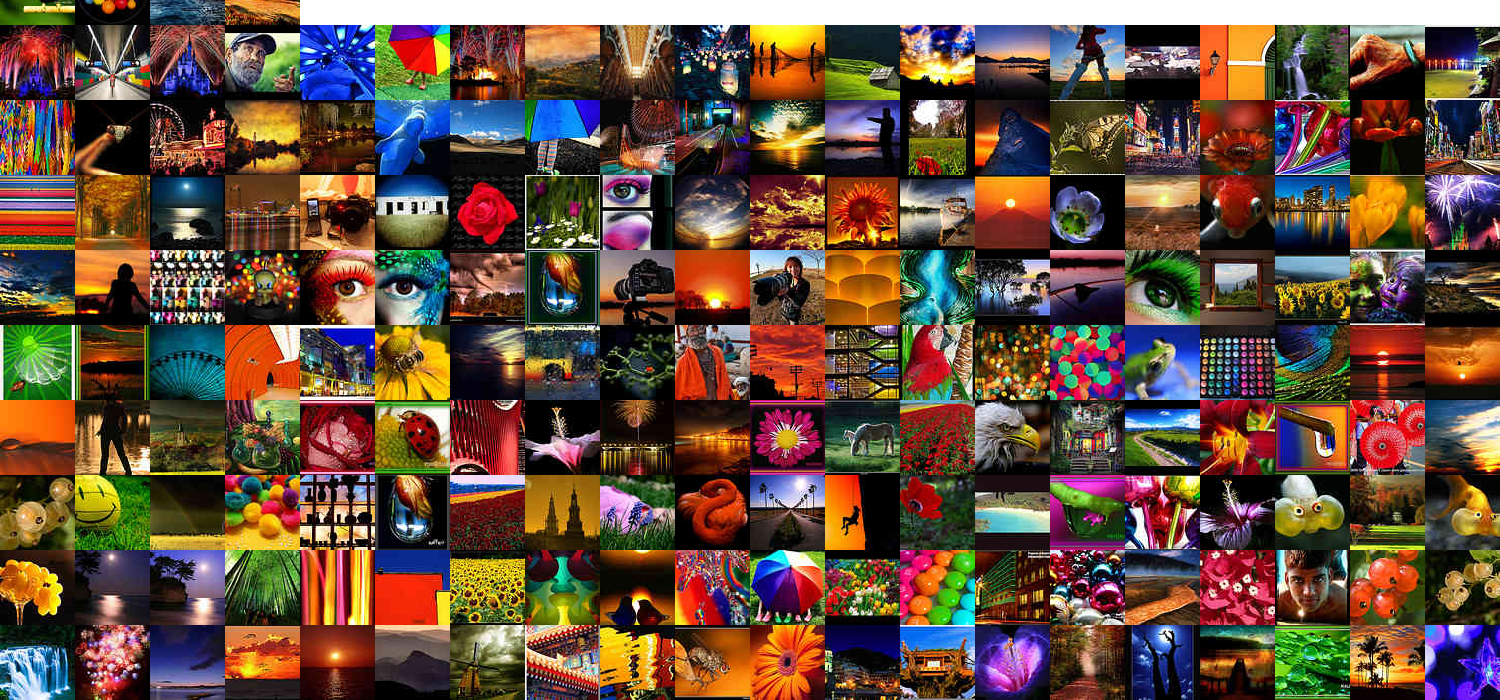
\includegraphics[height=0.25\textheight]{../../code/image_data/flickr_vivid_cluster_0.png}
    %\includegraphics[width=\textwidth]{flickr_vivid_clusters.pdf}
    \vskip20pt
    Represent each image with a binned RGB intensity histogram
  \end{center}

\end{frame}


\begin{frame}[fragile]
  \frametitle{Clustering images}

  \begin{center}

    \begin{block}{Group 'vivid' images into 3 clusters}
        \begin{lstlisting}[language=bash]
 ./cluster_flickr.py flickr_vivid 3 10
        \end{lstlisting}
    \end{block}
    \vskip20pt
    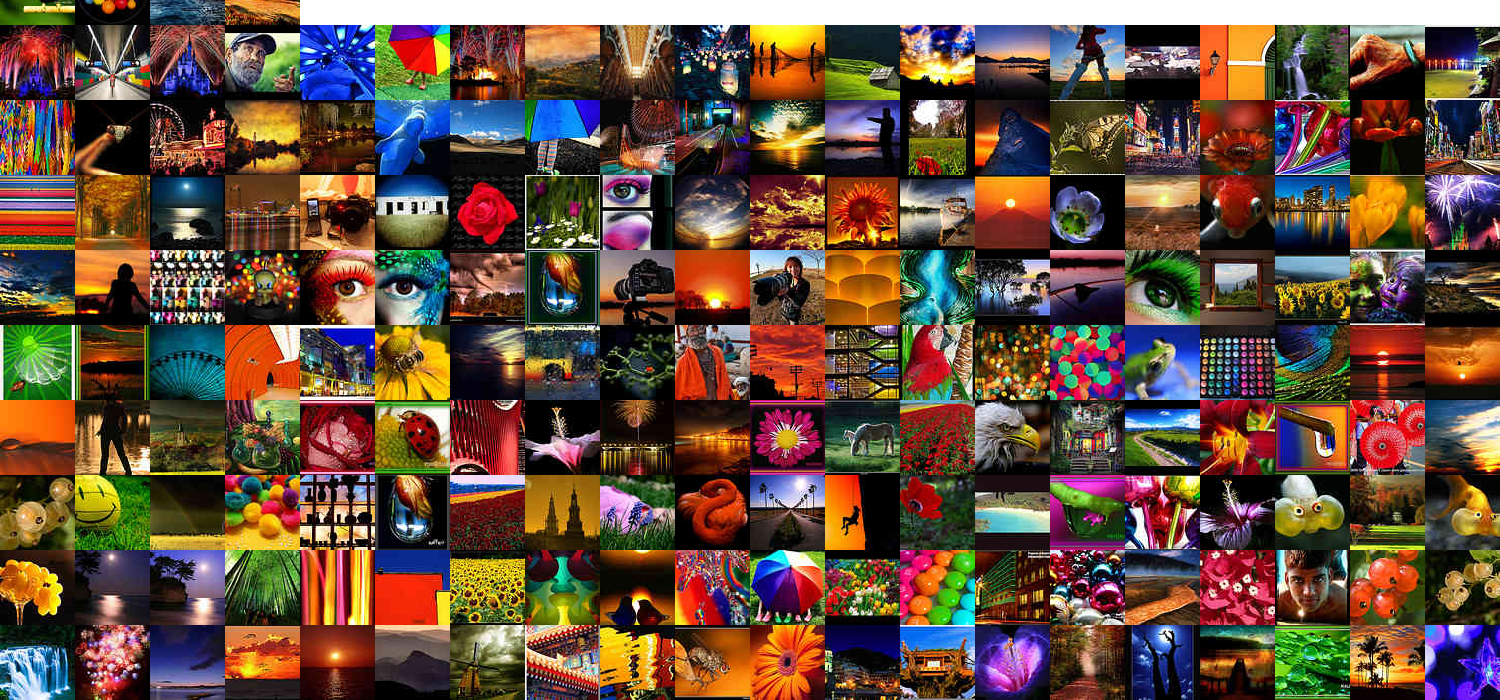
\includegraphics[height=0.2\textheight]{../../code/image_data/flickr_vivid_cluster_0.png}
    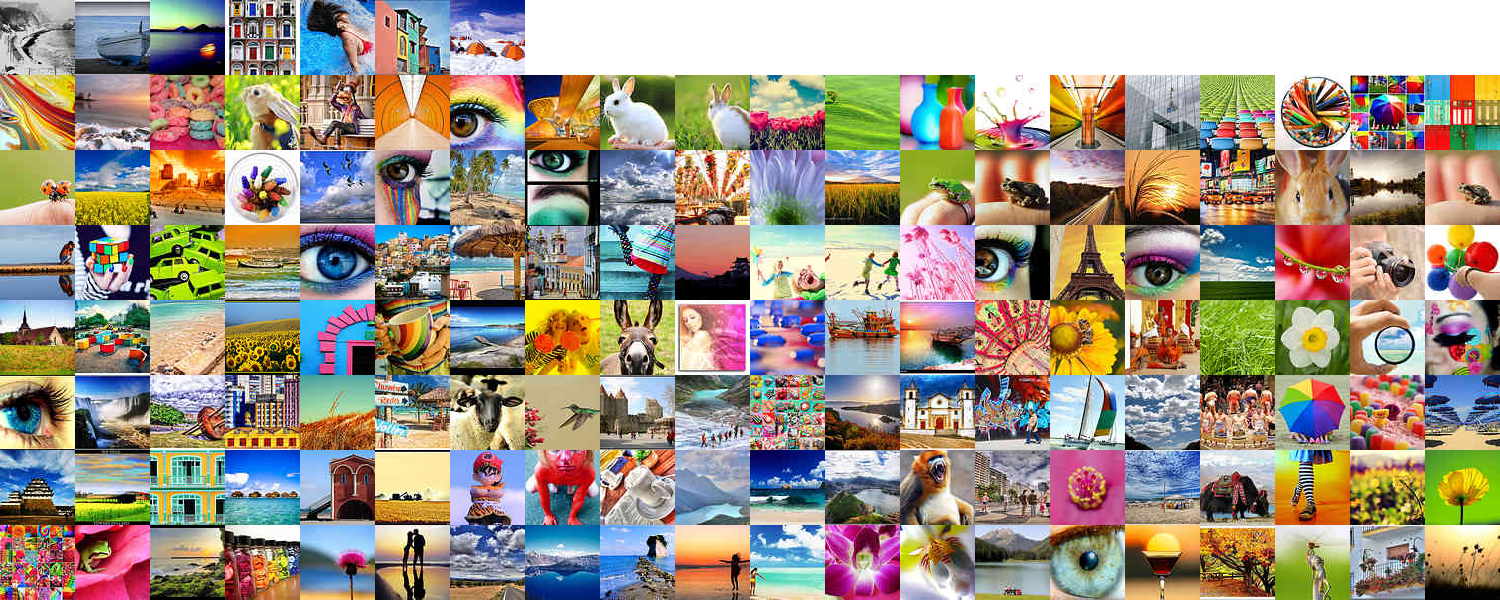
\includegraphics[height=0.2\textheight]{../../code/image_data/flickr_vivid_cluster_1.png}
    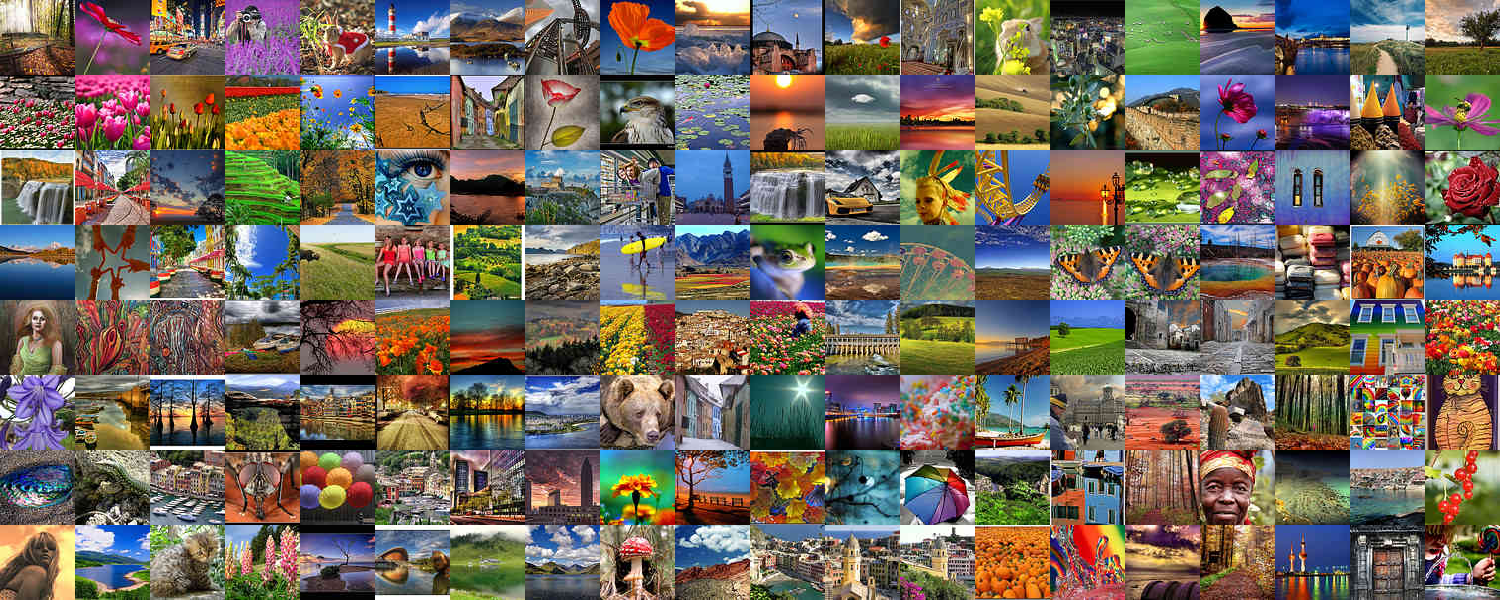
\includegraphics[height=0.2\textheight]{../../code/image_data/flickr_vivid_cluster_2.png}

  \end{center}

\end{frame}
